\documentclass[12pt,a4paper]{article}
\usepackage[utf8]{inputenc}
\usepackage[italian]{babel}
\usepackage{amsmath}
\usepackage{amsfonts}
\usepackage{amssymb}
\usepackage{graphicx}
\usepackage{siunitx}
\usepackage[left=2cm,right=2cm,top=2cm,bottom=0 cm]{geometry}
\newcommand{\rem}[1]{[\emph{#1}]}
\newcommand{\exn}{\phantom{xxx}}
\usepackage[italian]{babel}
\usepackage[utf8]{inputenc}
\usepackage{siunitx}
\usepackage{graphicx}
\usepackage{xcolor}
\usepackage{amsfonts}
\usepackage{amsmath}
\usepackage{amsthm}
\usepackage{tikz}
\usepackage{pgfplots}
\usepackage{enumitem}
\usepackage{subcaption}
\usepackage{siunitx}
\date{\today}
\usetikzlibrary{shapes.geometric,calc,matrix,arrows,snakes,shapes,patterns}
\title{Esercitazione 12B: Macchine e stati finiti:semaforo}
\author{Massimo Bilancioni, Alessandro Foligno, Giuseppe Zanichelli}
\begin{document}	
\maketitle
Si decide arbitrariamente di assegnare i vari stati di $Q_0$ e $Q_1$ ad altrettante posizioni del semaforo. In particolare, la corrispondenza scelta è:\\
\begin{enumerate}
	\item Lo stato (0,0) corrisponde al Verde
	\item Lo stato (0,1) corrisponde al Giallo+Verde
	\item Lo stato (1,0) corrisponde al Rosso
	\item Lo stato (1,1) corrisponde allo stato non desiderato che non rientra nel ciclo (in termini di colori per semplificare la  logica  l'abbiamo fatto corrispondere al Rosso+Giallo)
\end{enumerate}
Utilizzando questa corrispondenza, lo schema della transizione è riportato nella seguente tabella (insieme con i valori corrispondenti dei led)\
\begin{table}[h]\centering
\begin{tabular}{|c|c|c|c|c|c|c|}
	\hline 
	$Q_0^n$ & $Q_1^n$ & $Q_0^{n+1}$ & $Q_1^{n+1}$ & Verde & Giallo & Rosso \\ 
	\hline 
	0 & 0 & 0 & 1 & 1 & 0 & 0 \\ 
	\hline 
	0 & 1 & 1 & 0 & 1 & 1 & 0 \\ 
	\hline 
	1 & 0 & 0 & 0 & 0 & 0 & 1 \\ 
	\hline 
	1 & 1 & x & x & x & x & x \\ 
	\hline 
\end{tabular} 	
\caption{Tabella di transizione per $Q_0$ e $Q_1$}
\end{table}
\\
\noindent
osservando la tabella si vede che il segnale su Verde è proprio $\overline{Q_0}$ (ponendo $x =0$), quello su Giallo è $Q_1$ (ponendo $x= 1$), quello su Rosso è $Q_0$ (ponendo $x= 1$), questo è il motivo per cui abbiamo scelto che (1,1) corrisponde al Giallo+Rosso.\\
Per realizzare le transizioni, imponiamo che sia $Q_0^{n+1}=Q_1^n$ (ponendo $x= 1$)  e $Q_1^{n+1}=\overline{Q}_0^n \cdot \overline{Q}_1^n$ (ponendo $x= 0$), questo fa anche in modo che il valore di $(Q_0,Q_1)=(1,1)$ indesiderato non vada in se stesso.\\

Si riporta lo schema del circuito in Figura \ref{fig:circ} e la foto di quello realizzato in Figura \ref{fig:vg}; quest'ultima foto è stata fatta subito dopo aver acceso l'alimentazione e senza clock, come si vede sono accesi il led giallo e quello rosso e ci troviamo quindi inizialmente nello stato indesiderato. 
\begin{figure}[h]

			\centering

			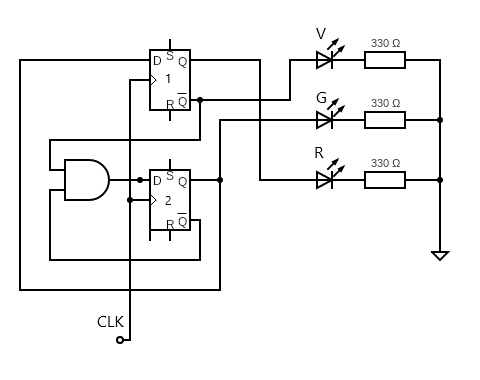
\includegraphics[scale=0.8]{circuit}

			\caption{ Schema circuito per l'implementazione del semaforo}

			\label{fig:circ}

\end{figure}

\begin{figure}[h]

			\centering

			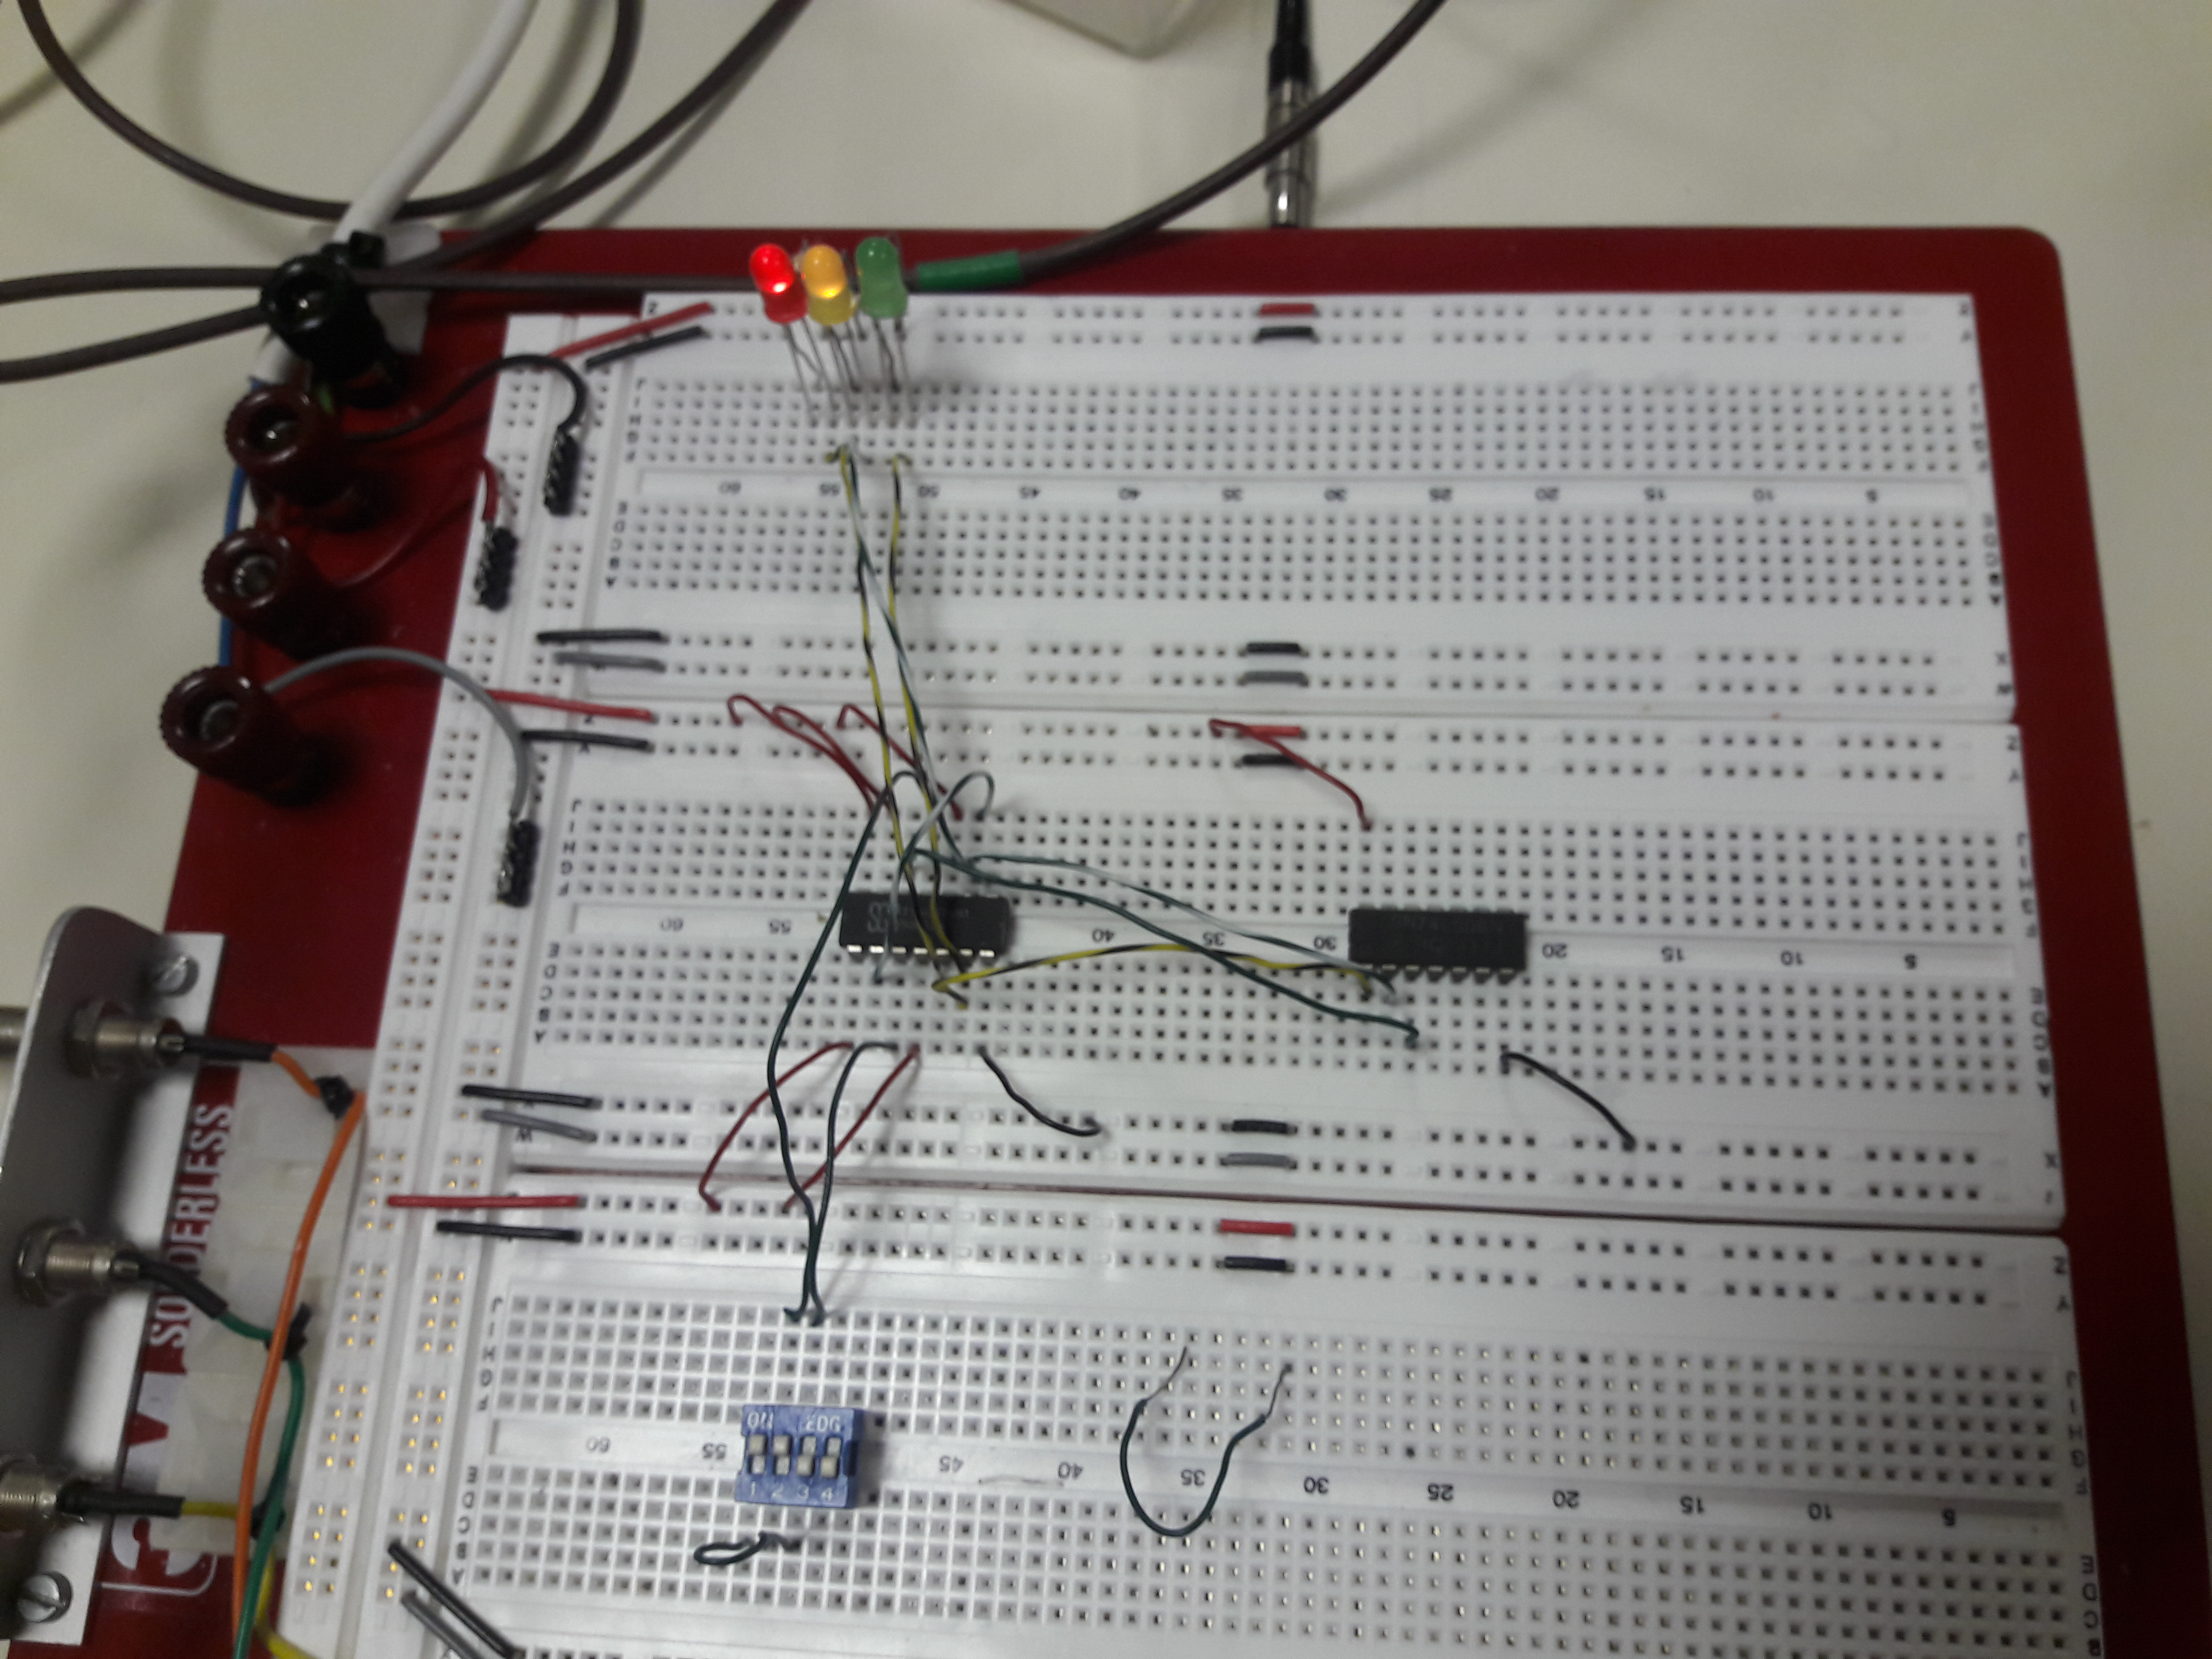
\includegraphics[scale=0.07]{gr}

			\caption{ Realizzazione circuito}

			\label{fig:vg}

\end{figure}



\newpage



\section{Forme d'onda}
Si osservano le seguenti forme d'onda sull'oscilloscopio (i commenti relativi sono sotto le varie figure):
\begin{figure}\centering
	\includegraphics[scale=0.9]{green.png}
	\caption{ segnale sul led verde (arancione) e del clock (blu), notare come il tempo in cui il verde sta acceso è il doppio di quello in cui è spento}
	
\end{figure}
\begin{figure}
	\centering
	\includegraphics[scale=0.8]{yellowandgreen.png}
	\includegraphics[scale=0.8]{yellowandred.png}
	
	\caption{il segnale in blu in entrambe  le figure corrisponde al led giallo, in arancio compaiono a sinistra  il segnale del led verde mentre a destra quello del led rosso. Notare che il giallo si accende solo quando il verde è  acceso e che il verde e il rosso (ovvero i due segnali arancioni) sono complementari}
	
\end{figure}
\begin{figure}
\centering

\includegraphics[scale=0.8]{Q1andQ2}
\caption{sono mostrati i segnali Q0 e Q1 che compiono come desiderato il ciclo di  transizioni $00\to 01 \to 10 \to 00$}
\end{figure}

\end{document}